\xchapter{PRIEDAI}

\xsection{Priedas nr. 1: Klausimynas prieš testavimą}
\noindent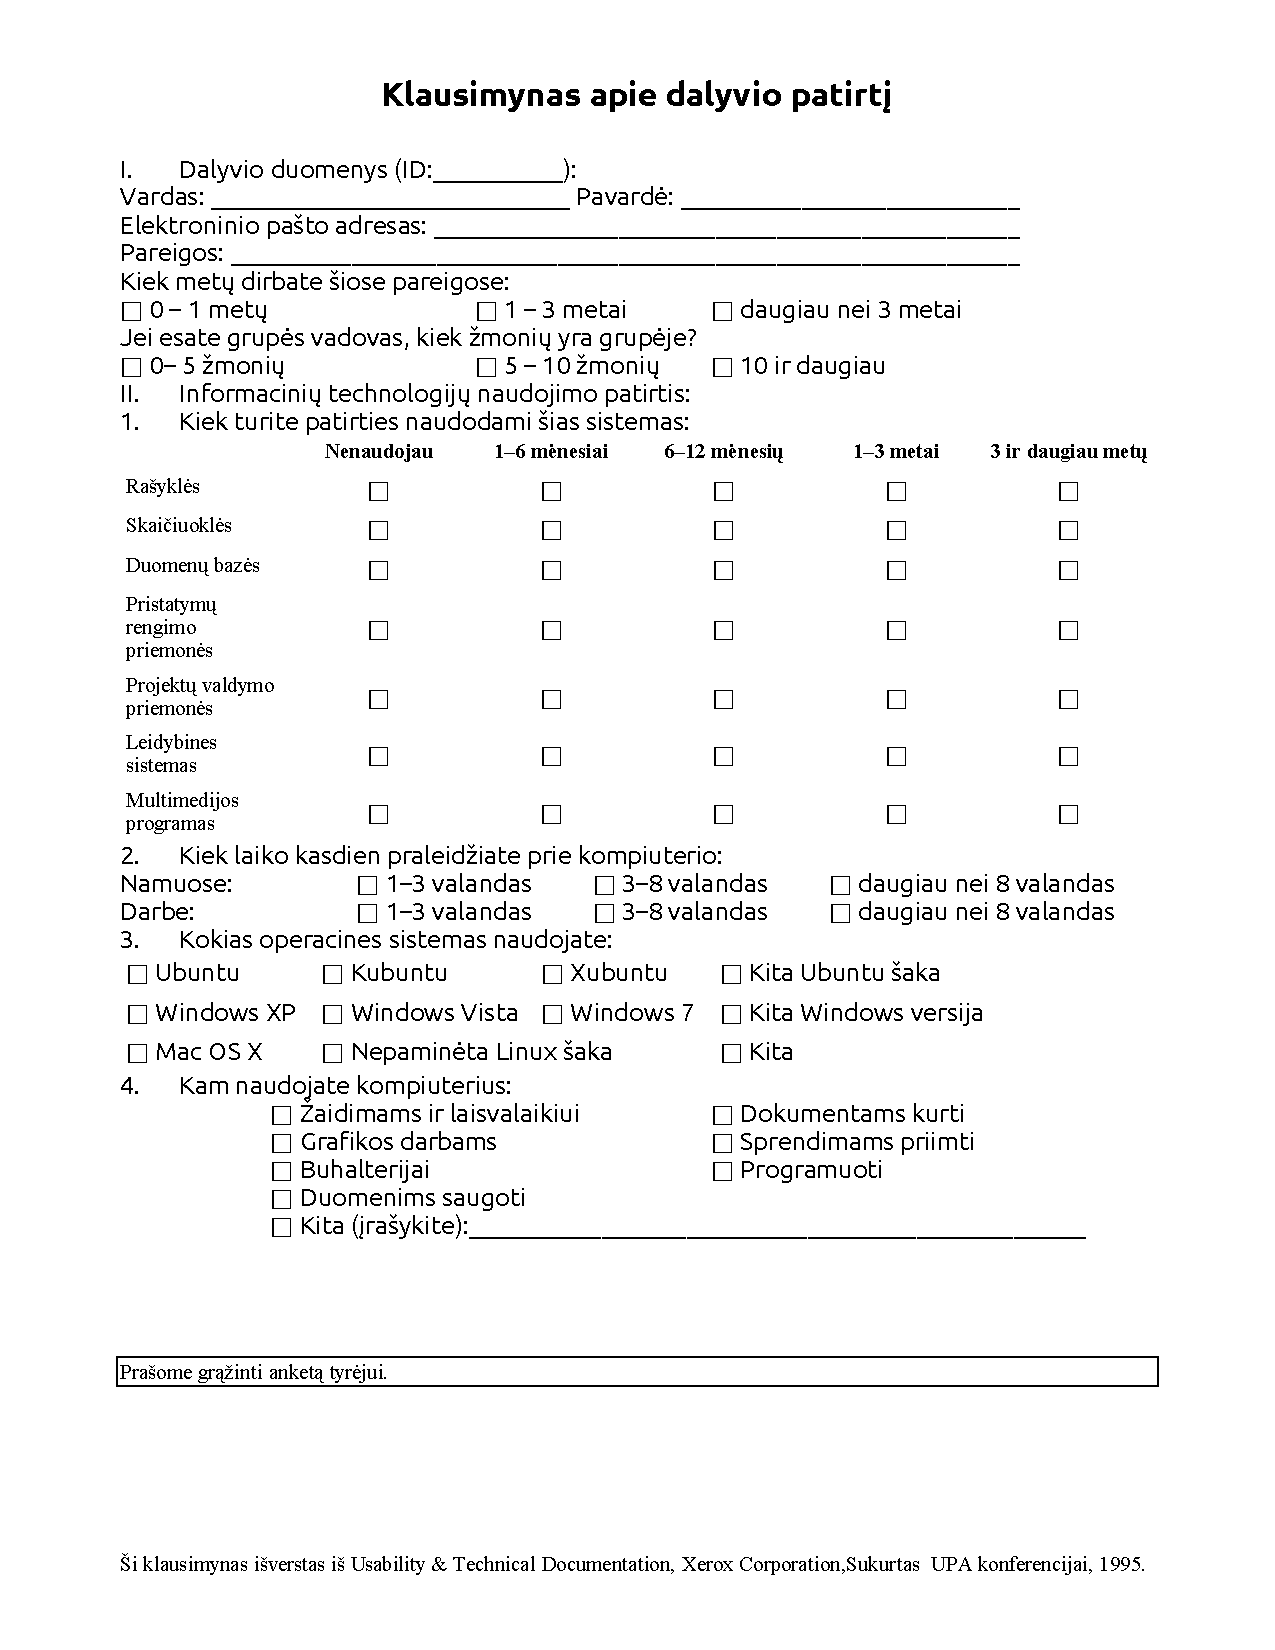
\includegraphics[scale=0.75]{./4/pdfs/klausimynas0.pdf}

\xsection{Priedas nr. 2: Klausimynas po testavimo}
\noindent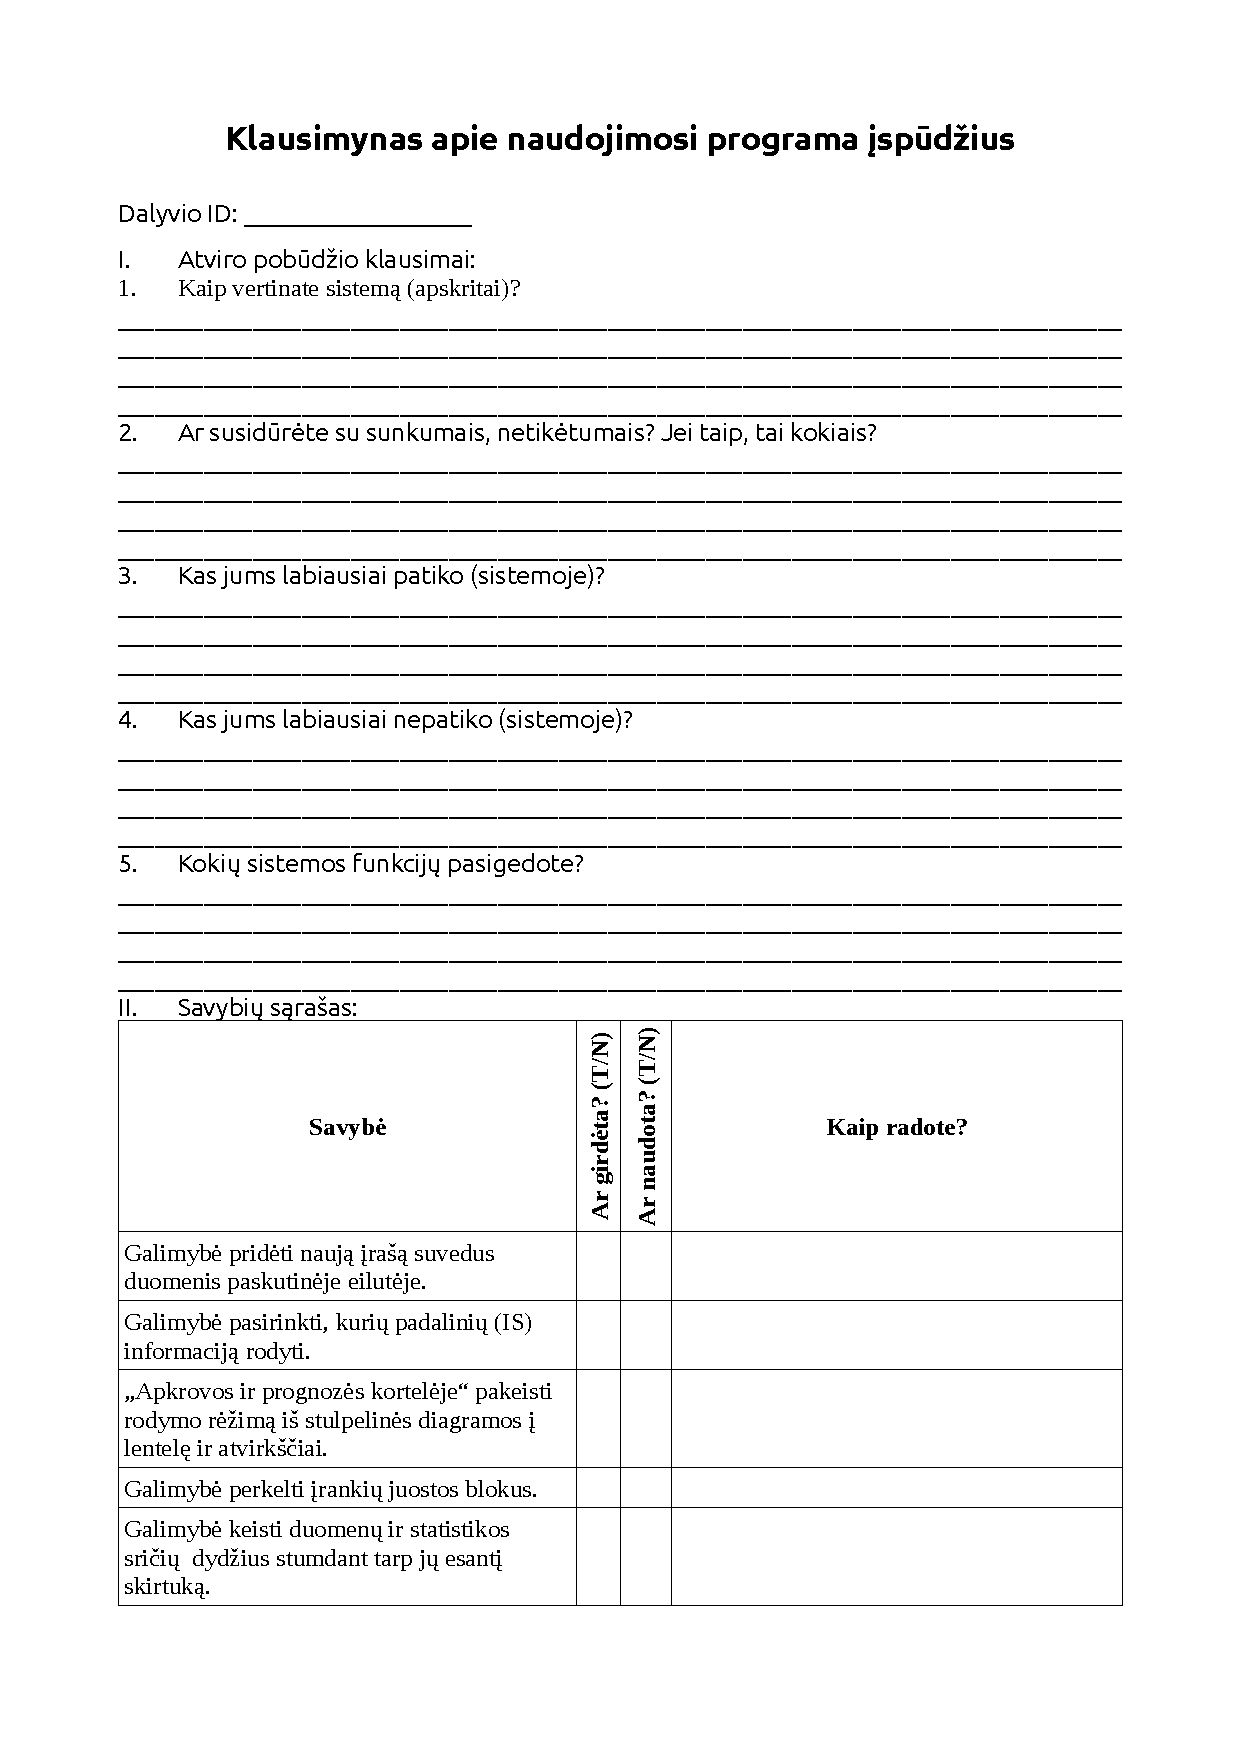
\includegraphics[scale=0.85, page=1]{./4/pdfs/klausimynas1.pdf}

\newpage
\noindent\includegraphics[scale=0.85, page=2]{./4/pdfs/klausimynas1.pdf}

\newpage
\noindent\includegraphics[scale=0.85, page=3]{./4/pdfs/klausimynas1.pdf}

TODO: Pridėti sutikimo formą.

TODO: Pridėti užduoties aprašymą.

\newpage
\xsection{Priedas nr. 3: Dalyvių rezultatų lentelės}

TODO: DĖSTYTOJA: Kas turėtų būti čia? Spėjimas:
\begin{itemize}
  \item kiek laiko kuris testuotojas užtruko kurios dalies vykdymui;
  \item kurias dalis testuotojui pavyko sėkmingai atlikti;
  \item jei nepavyko, tai kodėl.
\end{itemize}
